\documentclass[a4paper,11pt]{article}
\usepackage[utf8]{inputenc}
\usepackage{geometry}
\usepackage{graphicx}
\usepackage{listings}
\usepackage{xcolor}
\usepackage{tikz}
\usetikzlibrary{shapes.geometric, arrows, positioning, fit, calc}

\geometry{left=2cm,right=2cm,top=2cm,bottom=2cm}
\definecolor{backcolour}{rgb}{0.95,0.95,0.92}
\definecolor{codepurple}{rgb}{0.58,0,0.82}
\definecolor{codeblue}{rgb}{0.1,0.1,0.6}

\lstdefinestyle{pythonstyle}{
    backgroundcolor=\color{backcolour},   
    commentstyle=\color{gray},
    keywordstyle=\color{codeblue}\bfseries,
    numberstyle=\tiny\color{gray},
    stringstyle=\color{codepurple},
    basicstyle=\ttfamily\small,
    breakatwhitespace=false,         
    breaklines=true,                 
    captionpos=b,                    
    keepspaces=true,                 
    numbers=left,                    
    numbersep=5pt,                  
    showspaces=false,                
    showstringspaces=false,
    showtabs=false,                  
    tabsize=4,
    frame=lines
}
\lstset{style=pythonstyle}

\title{\textbf{Practical Work 4: Word Count}}
\author{Group 16}
\date{\today}

\begin{document}

\maketitle

\section{Overview}
The objective of this lab is to implement the \textbf{Word Count} algorithm using the MapReduce paradigm. This serves as a fundamental example to understand how large datasets are processed in distributed systems by counting the frequency of every word in a text corpus.

\section{Implementation Strategy}
We decided to implement a custom MapReduce framework using \textbf{Python's Multiprocessing} module.

\subsection{Why this implementation?}
Instead of a simple sequential simulation, we chose \textbf{Multiprocessing} to mimic a real cluster environment:
\begin{itemize}
    \item \textbf{Parallelism:} Each Mapper runs in a separate system process (Worker), utilizing different CPU cores. This demonstrates the "Scale-out" philosophy of MapReduce.
    \item \textbf{Independence:} Each worker processes its data chunk independently without sharing memory, enforcing the strict functional programming constraints of MapReduce.
    \item \textbf{Scalability:} The number of workers can be adjusted to match the hardware capabilities (e.g., 2, 4, or 8 workers).
\end{itemize}

\section{System Architecture}

\subsection{Data Flow Diagram}
The following figure illustrates the horizontal data flow from raw text to the final aggregate count.

\begin{figure}[h]
    \centering
    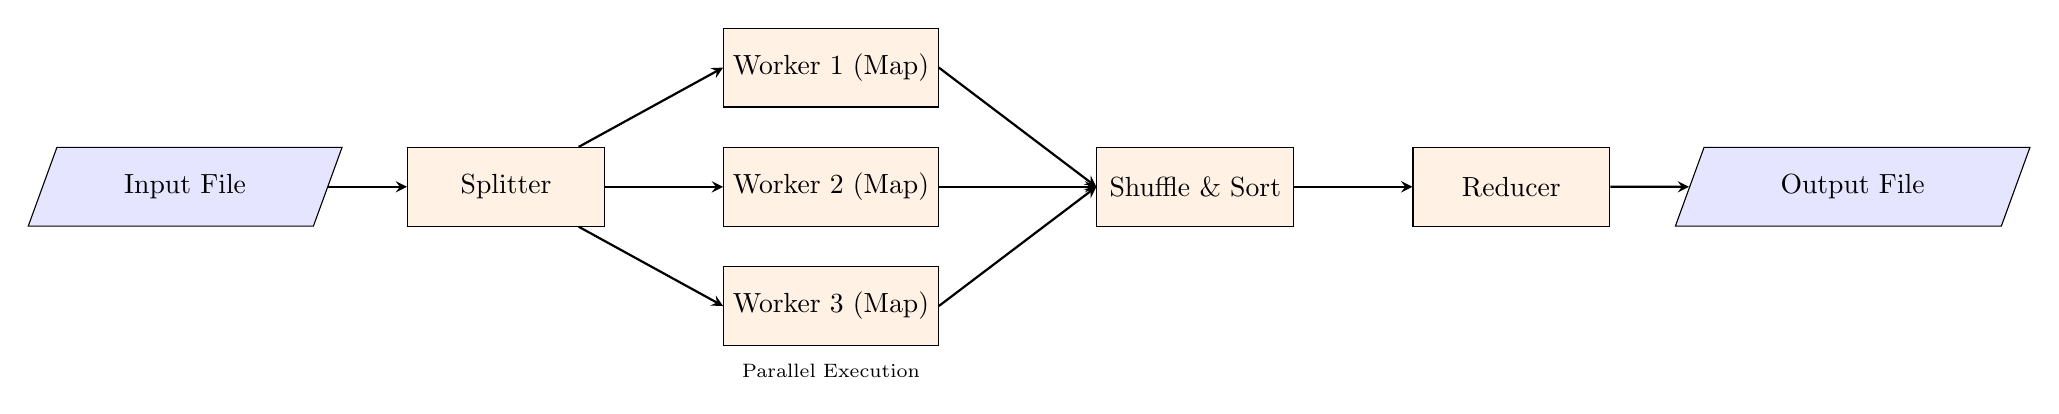
\begin{tikzpicture}[
        node distance=2cm,
        startstop/.style={rectangle, rounded corners, minimum width=2cm, minimum height=1cm,text centered, draw=black, fill=red!10},
        process/.style={rectangle, minimum width=2.5cm, minimum height=1cm, text centered, draw=black, fill=orange!10},
        io/.style={trapezium, trapezium left angle=70, trapezium right angle=110, minimum width=2cm, minimum height=1cm, text centered, draw=black, fill=blue!10},
        arrow/.style={thick,->,>=stealth}
    ]

    \node (input) [io] {Input File};
    \node (split) [process, right=1cm of input] {Splitter};
    
    \node (map1) [process, above right=0.5cm and 1.5cm of split] {Worker 1 (Map)};
    \node (map2) [process, right=1.5cm of split] {Worker 2 (Map)};
    \node (map3) [process, below right=0.5cm and 1.5cm of split] {Worker 3 (Map)};
    
    \node (shuffle) [process, right=2cm of map2] {Shuffle \& Sort};
    \node (reduce) [process, right=1.5cm of shuffle] {Reducer};
    \node (output) [io, right=1cm of reduce] {Output File};

    \draw [arrow] (input) -- (split);
    \draw [arrow] (split) -- (map1.west);
    \draw [arrow] (split) -- (map2.west);
    \draw [arrow] (split) -- (map3.west);
    
    \draw [arrow] (map1.east) -- (shuffle.west);
    \draw [arrow] (map2.east) -- (shuffle.west);
    \draw [arrow] (map3.east) -- (shuffle.west);
    
    \draw [arrow] (shuffle) -- (reduce);
    \draw [arrow] (reduce) -- (output);
    
    \node [below=0.1cm of map3, font=\scriptsize] {Parallel Execution};

    \end{tikzpicture}
    \caption{MapReduce Execution Flow}
    \label{fig:mr_flow}
\end{figure}

\subsection{Mapper Logic}
The mapper uses Regular Expressions (`re` module) to cleanly tokenize words, handling punctuation and case sensitivity automatically.

\begin{lstlisting}[language=Python, caption=Mapper Worker]
def map_worker(text_chunk):
    # Find all words using regex boundary
    words = re.findall(r'\b\w+\b', text_chunk.lower())
    return [(word, 1) for word in words]
\end{lstlisting}

\subsection{Reducer Logic}
The reducer is a simple aggregation function that sums the list of ones generated by the mappers.

\begin{lstlisting}[language=Python, caption=Reducer Logic]
def reduce_worker(item):
    word, counts = item
    # Summing the occurrences
    return (word, sum(counts))
\end{lstlisting}

\section{Task Allocation}
\begin{table}[h]
\centering
\begin{tabular}{|l|l|p{6cm}|}
\hline
\textbf{Member} & \textbf{Role} & \textbf{Responsibilities} \\ \hline
Member 1 & Core Dev & Implementing Multiprocessing Pool and Map logic. \\ \hline
Member 2 & Data Dev & Implementing Shuffle/Sort logic and File I/O handling. \\ \hline
Member 3 & Reporter & Designing the LaTeX report and TikZ Architecture diagram. \\ \hline
\end{tabular}
\caption{Team Responsibilities}
\end{table}

\end{document}